\documentclass{beamer}
\usetheme{Madrid}
%\usepackage[orientation=landscape,size=custom,width=28,height=21,scale=1,debug]{beamerposter} 
% width=11.333,height=8.5
\geometry{paperwidth=8.5in,paperheight=4.75in} 
% paperwidth=11.333in,paperheight=8.5in

%	%%%%%%%%%%%%%	%
% Load packages %
%	%%%%%%%%%%%%%	%

%\usepackage{helvet}
%\usepackage{tikz}
%\usepackage{lmodern} % Load Latin Modern fonts
%\usepackage{subcaption}
%\usepackage{multirow}
\usepackage{booktabs} % For better table rules
%\usepackage{graphicx} % for including graphics
%\usepackage{multicol}
%\usepackage{amsmath}
\usepackage[citestyle=authoryear, bibstyle=authoryear, sorting=nyt]{biblatex}
\AtEveryBibitem{
	\clearfield{issn}
	\ifentrytype{book}{\clearfield{isbn}}{}
    \clearfield{urlyear}
    \clearfield{urlmonth}
    \clearfield{urlday}
}
\addbibresource{../ps_honors_thesis.bib}

%----- Beamer options -----%
\AtBeginSection[]
{
  \begin{frame}
    \frametitle{Table of Contents}
    \tableofcontents[currentsection]
  \end{frame}
}

%\setbeameroption{hide notes} % Only slides
%\setbeameroption{show only notes} % Only notes
\setbeameroption{show notes on second screen=right} % Both
\setbeamertemplate{navigation symbols}{} % No navigation buttons

\setbeamercolor{frametitle}{bg=cyan!7, fg=black}

% Redefine bibliography colors to black
\setbeamercolor{bibliography entry author}{fg=black}
\setbeamercolor{bibliography entry title}{fg=black} % Set book titles to black
\setbeamercolor{bibliography entry note}{fg=black}
\setbeamercolor{caption name}{fg=black}
\setbeamercolor{title}{bg=cyan!7, fg=black}
\setbeamercolor{subtitle}{bg=white, fg=black}

\setbeamerfont{bibliography entry author}{size=\small}
\setbeamerfont{bibliography entry title}{size=\small}
\setbeamerfont{bibliography entry note}{size=\small}
\setbeamerfont{caption name}{size=\small}

\title{The Policing of the “Reserve Army”}
\subtitle{Economic Inequality and Police Killings}
\author{Matthew A. Carson}\date{May 21, 2024}

\begin{document}

\begin{frame}
  \titlepage
  \note[item]{Welcome to the talk!}
\end{frame}

\section{Research Question and Design}
%----- Research Question -----%
\begin{frame}{Research Question}
	\begin{itemize}
		\item How does class, economic inequality, and gentrification contribute to the incidence of police killings in the US? \pause
		\begin{itemize}
			\item There are sharp racial disparities.
			\item But what are the economic dimensions? \pause
			\begin{itemize}
				\item I'm interested specifically in looking at place. \pause
			\end{itemize}
			\item How do processes of gentrification contribute to rates of police killings?
		\end{itemize}		
	\end{itemize}
\end{frame}

%----- Research Design -----%
\begin{frame}{Research Design: Data Sources}
	\begin{itemize}
	\item US Census American Community Survey
		\begin{itemize}
			\item Median Family Income in tracts
			\item Racial composition of tracts
		\end{itemize} \pause
	\item FatalEncounters.org
		\begin{itemize}
			\item List of people killed by law enforcement in the US
			\item Compiled by journalists -- FBI data not reliable
			\item Years in this study 2015--2020, inclusive.
		\end{itemize} \pause
	\item Urban Displacement Project Typologies \nocite{udpDisplacementGentrificationTypologies2023}
		\begin{itemize}
			\item Condensed into three typologies
			\begin{itemize}
				\item Low-Income or At-Risk
				\item Gentrifying
				\item Stable
			\end{itemize}
		\end{itemize}
	\end{itemize}
\end{frame}

\begin{frame}{Research Design: Definitions}
	\begin{itemize}
		\item Lethal Use of Force (LUOF)
		\begin{itemize}
			\item Include
			\begin{itemize}
				\item  tasered, gunshot, stabbed, asphyxiated/restrained, beaten/bludgeoned with an instrument, chemical agent/pepper spray, asphyxiation/restrained, or less than lethal force.
			\end{itemize}
			\item Exclude
			\begin{itemize}
				\item vehicle, fell from a height, drowned, medical emergency, other, burned/smoke inhalation, drug overdose, and undetermined.
			\end{itemize}
		\end{itemize}
	\end{itemize}
\end{frame}

\begin{frame}{Research Design: Gentrification}
\begin{center}
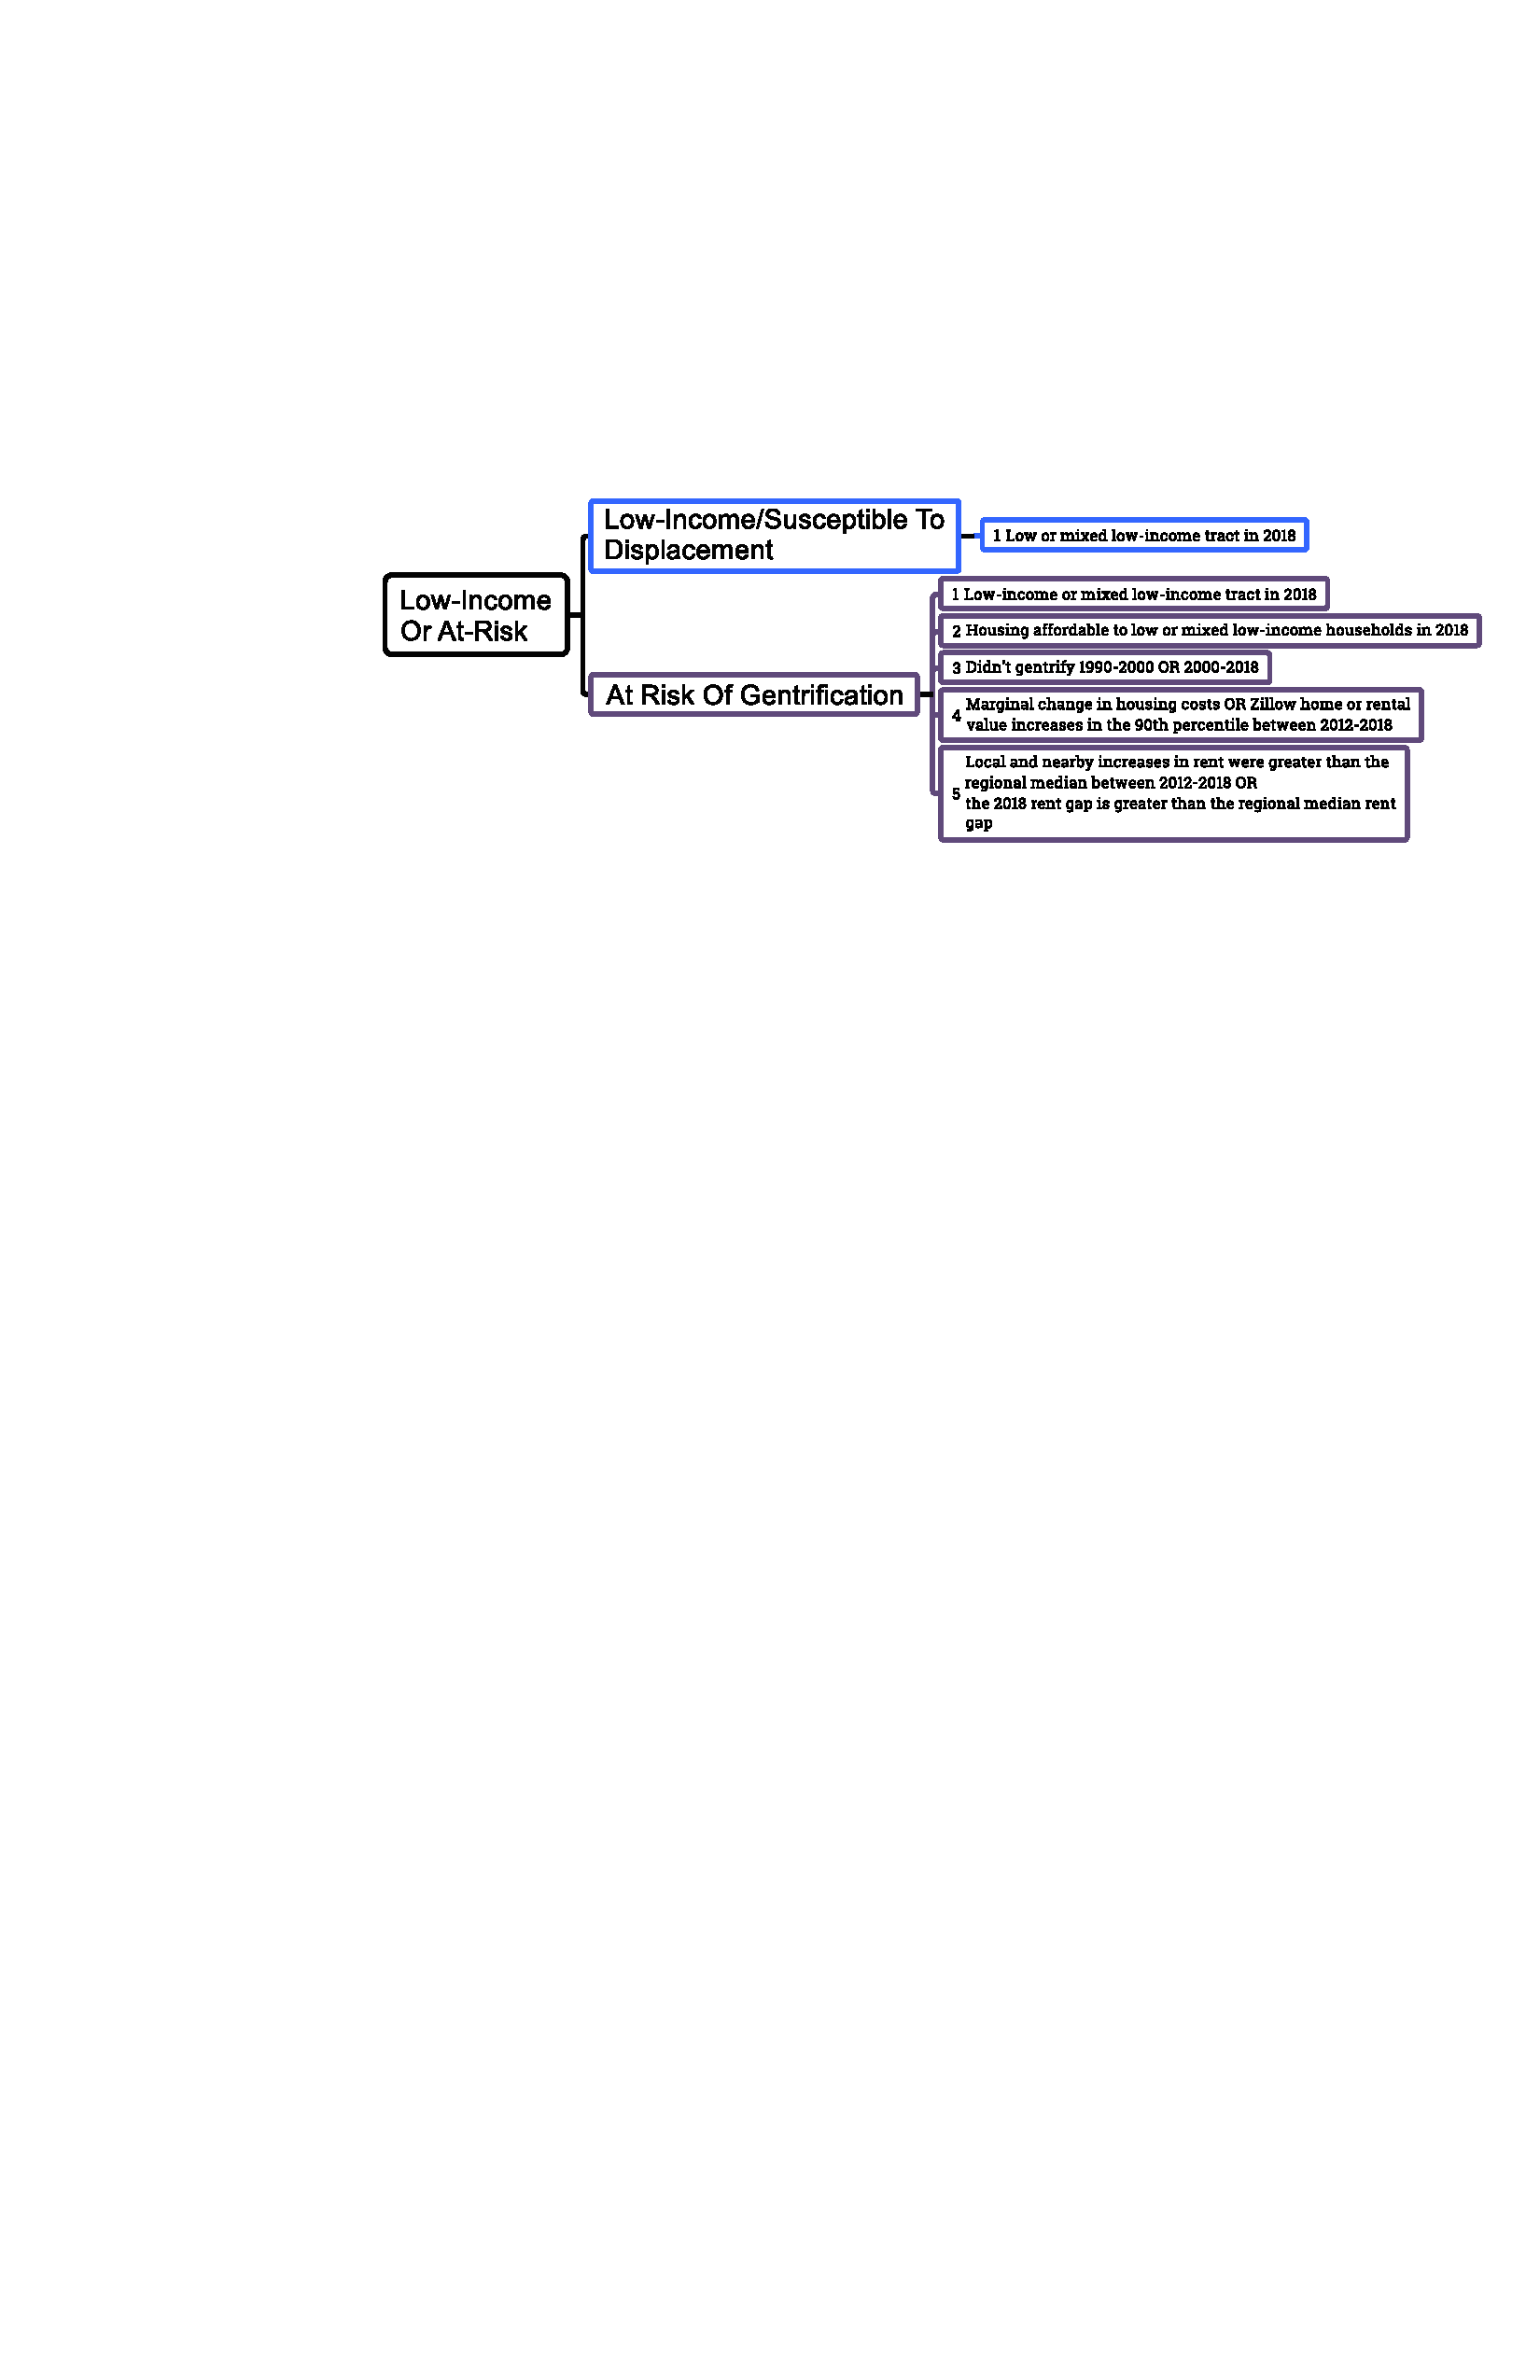
\includegraphics[scale=1]{images/low_income_at_risk}
\end{center}
\end{frame}

\begin{frame}{Research Design: Gentrification}
\begin{center}
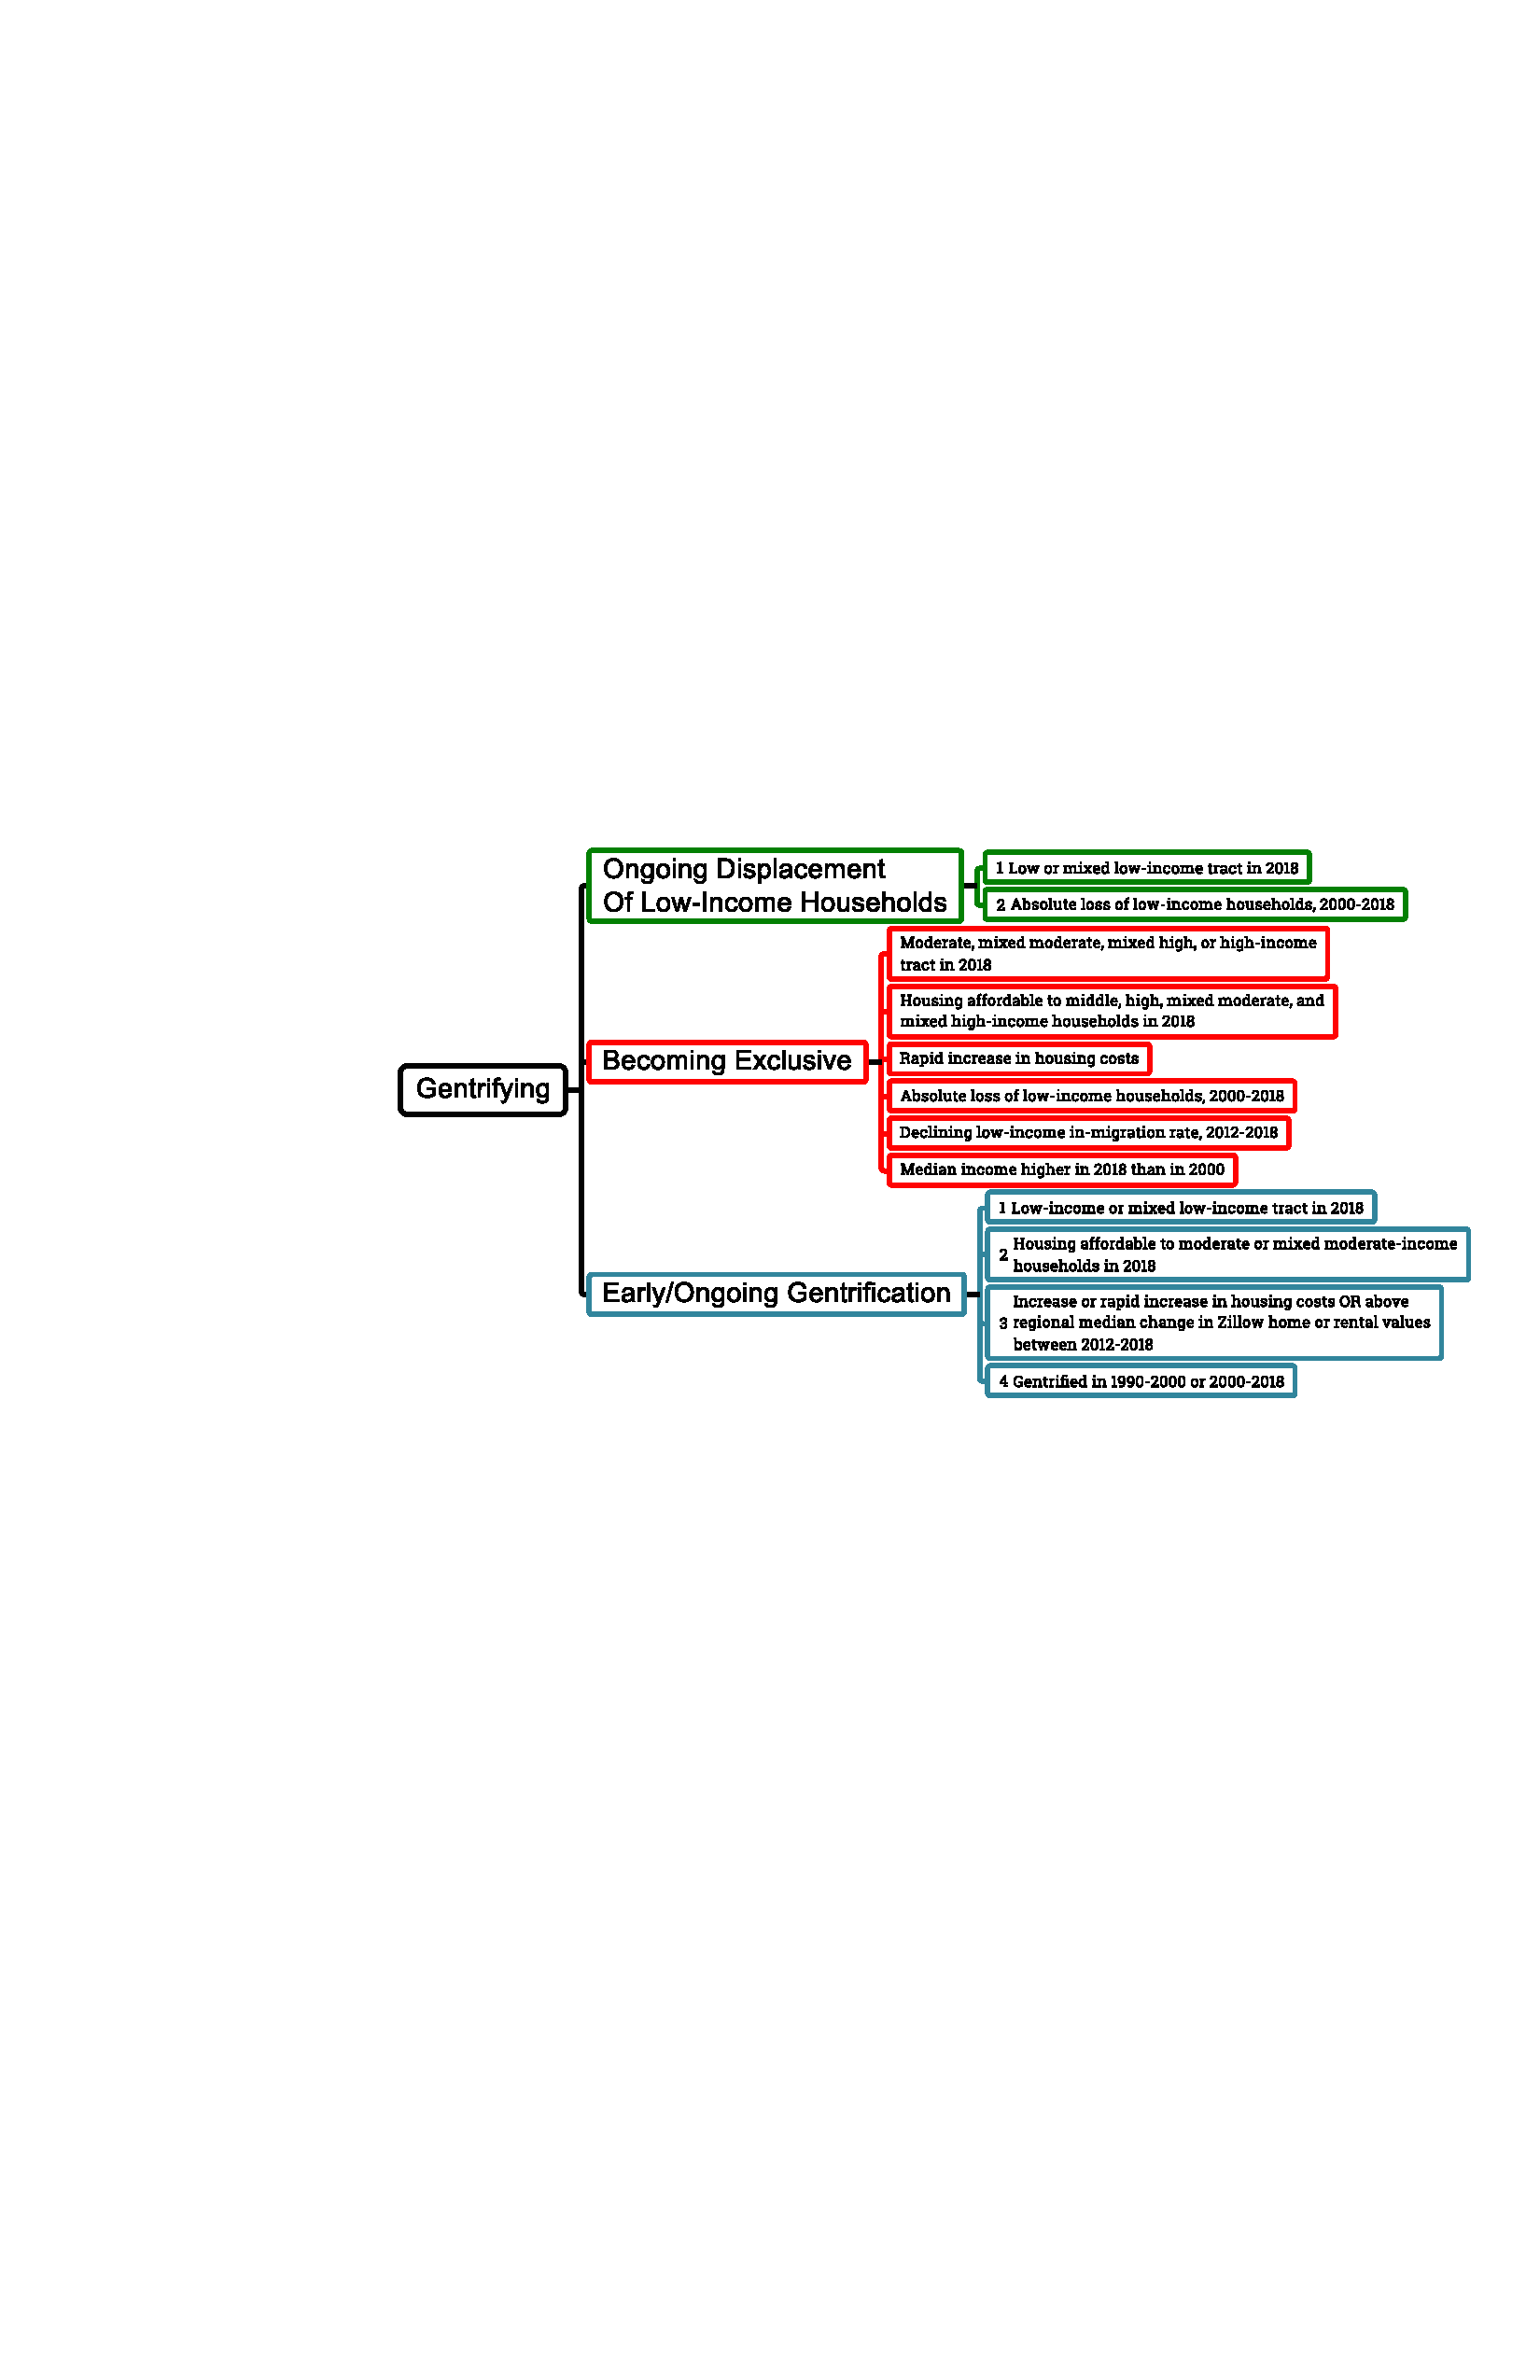
\includegraphics[scale=1]{images/gentrifying}
\end{center}
\end{frame}

\begin{frame}{Research Design: Gentrification}
\begin{center}
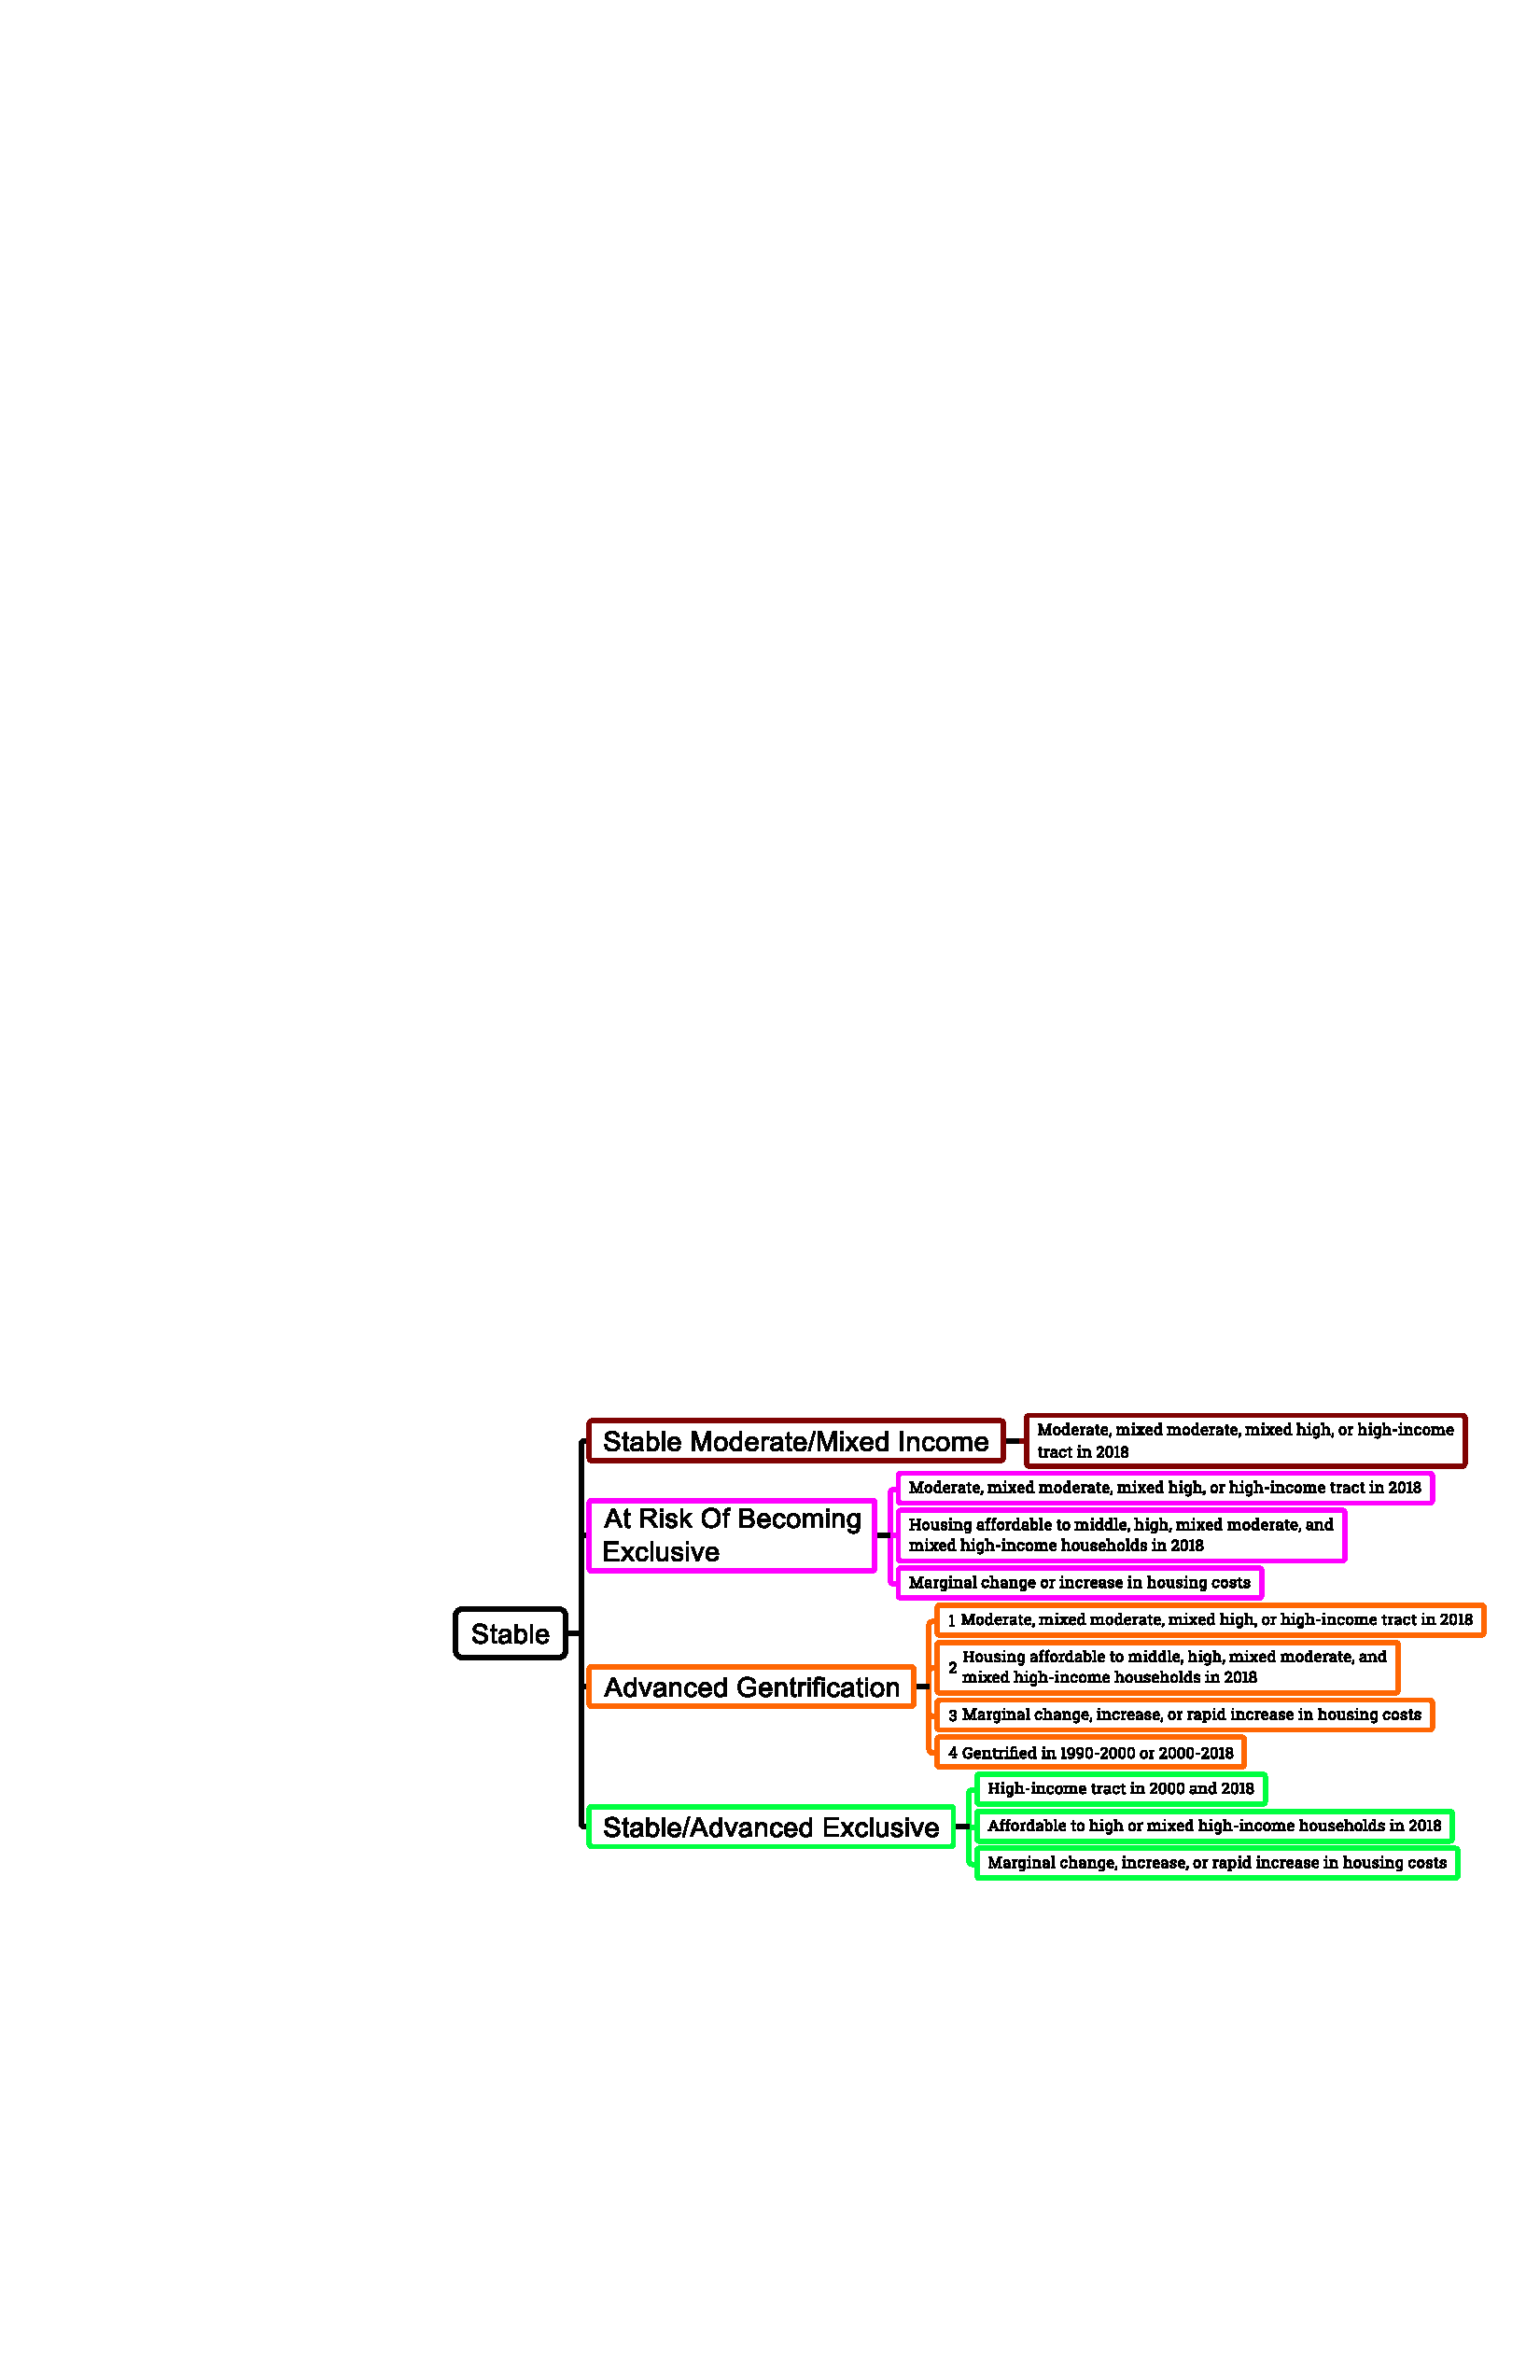
\includegraphics[scale=1]{images/stable}
\end{center}
\end{frame}

\begin{frame}{Research Design: Hypotheses}
	\begin{tabular}{@{} l @{\hspace{18pt}} p{432pt} @{}}
	$\textbf{H}_1$: & LUOF rates should vary more substantially by income quintiles within each racial group than by racial groups within each income quintile. The lowest income quintiles should have the highest LUOF rates.
	\end{tabular}
	\vfill
	\begin{tabular}{@{} l @{\hspace{18pt}} p{432pt} @{}}
	$\textbf{H}_2$: &Tracts experiencing gentrification or vulnerable to becoming gentrified should experience higher rates of LUOF than higher-income tracts that have experienced no gentrification, regardless of the racial composition of the tract. That is, there should be more variation within each racial group by gentrification typology than there is within each gentrification typology by majority race.
	\end{tabular}
\end{frame}

\section{Literature Review}
%---- Literature Review ------%
\begin{frame}{Literature Review}
	\begin{itemize}
		\item Quantitative
		\begin{itemize}
			\item \textcite{feldmanPoliceRelatedDeathsNeighborhood2019}
			\item \textcite{feldmanPoliceKillingsUS2020} \pause
		\end{itemize}
		\item Historical
		\begin{itemize}
			\item \citeauthor{johnsonAfterwordBaltimorePolicing2016} \parencites*{
			johnsonAfterwordBaltimorePolicing2016, 
			johnsonTrumpismPolicingProblem2019, 
			johnsonBlackLivesMatter2023} \pause
		\end{itemize}
		\item Space \& Place
		\begin{itemize}
			\item \textcite{wacquantClassRaceHyperincarceration2010}
		\end{itemize}
	\end{itemize}
\end{frame}

%----- Findings -----%
\section{Findings: Race and Tract Income}
\begin{frame}{Findings: Rates by Race/Ethnicity}
	\begin{center}
	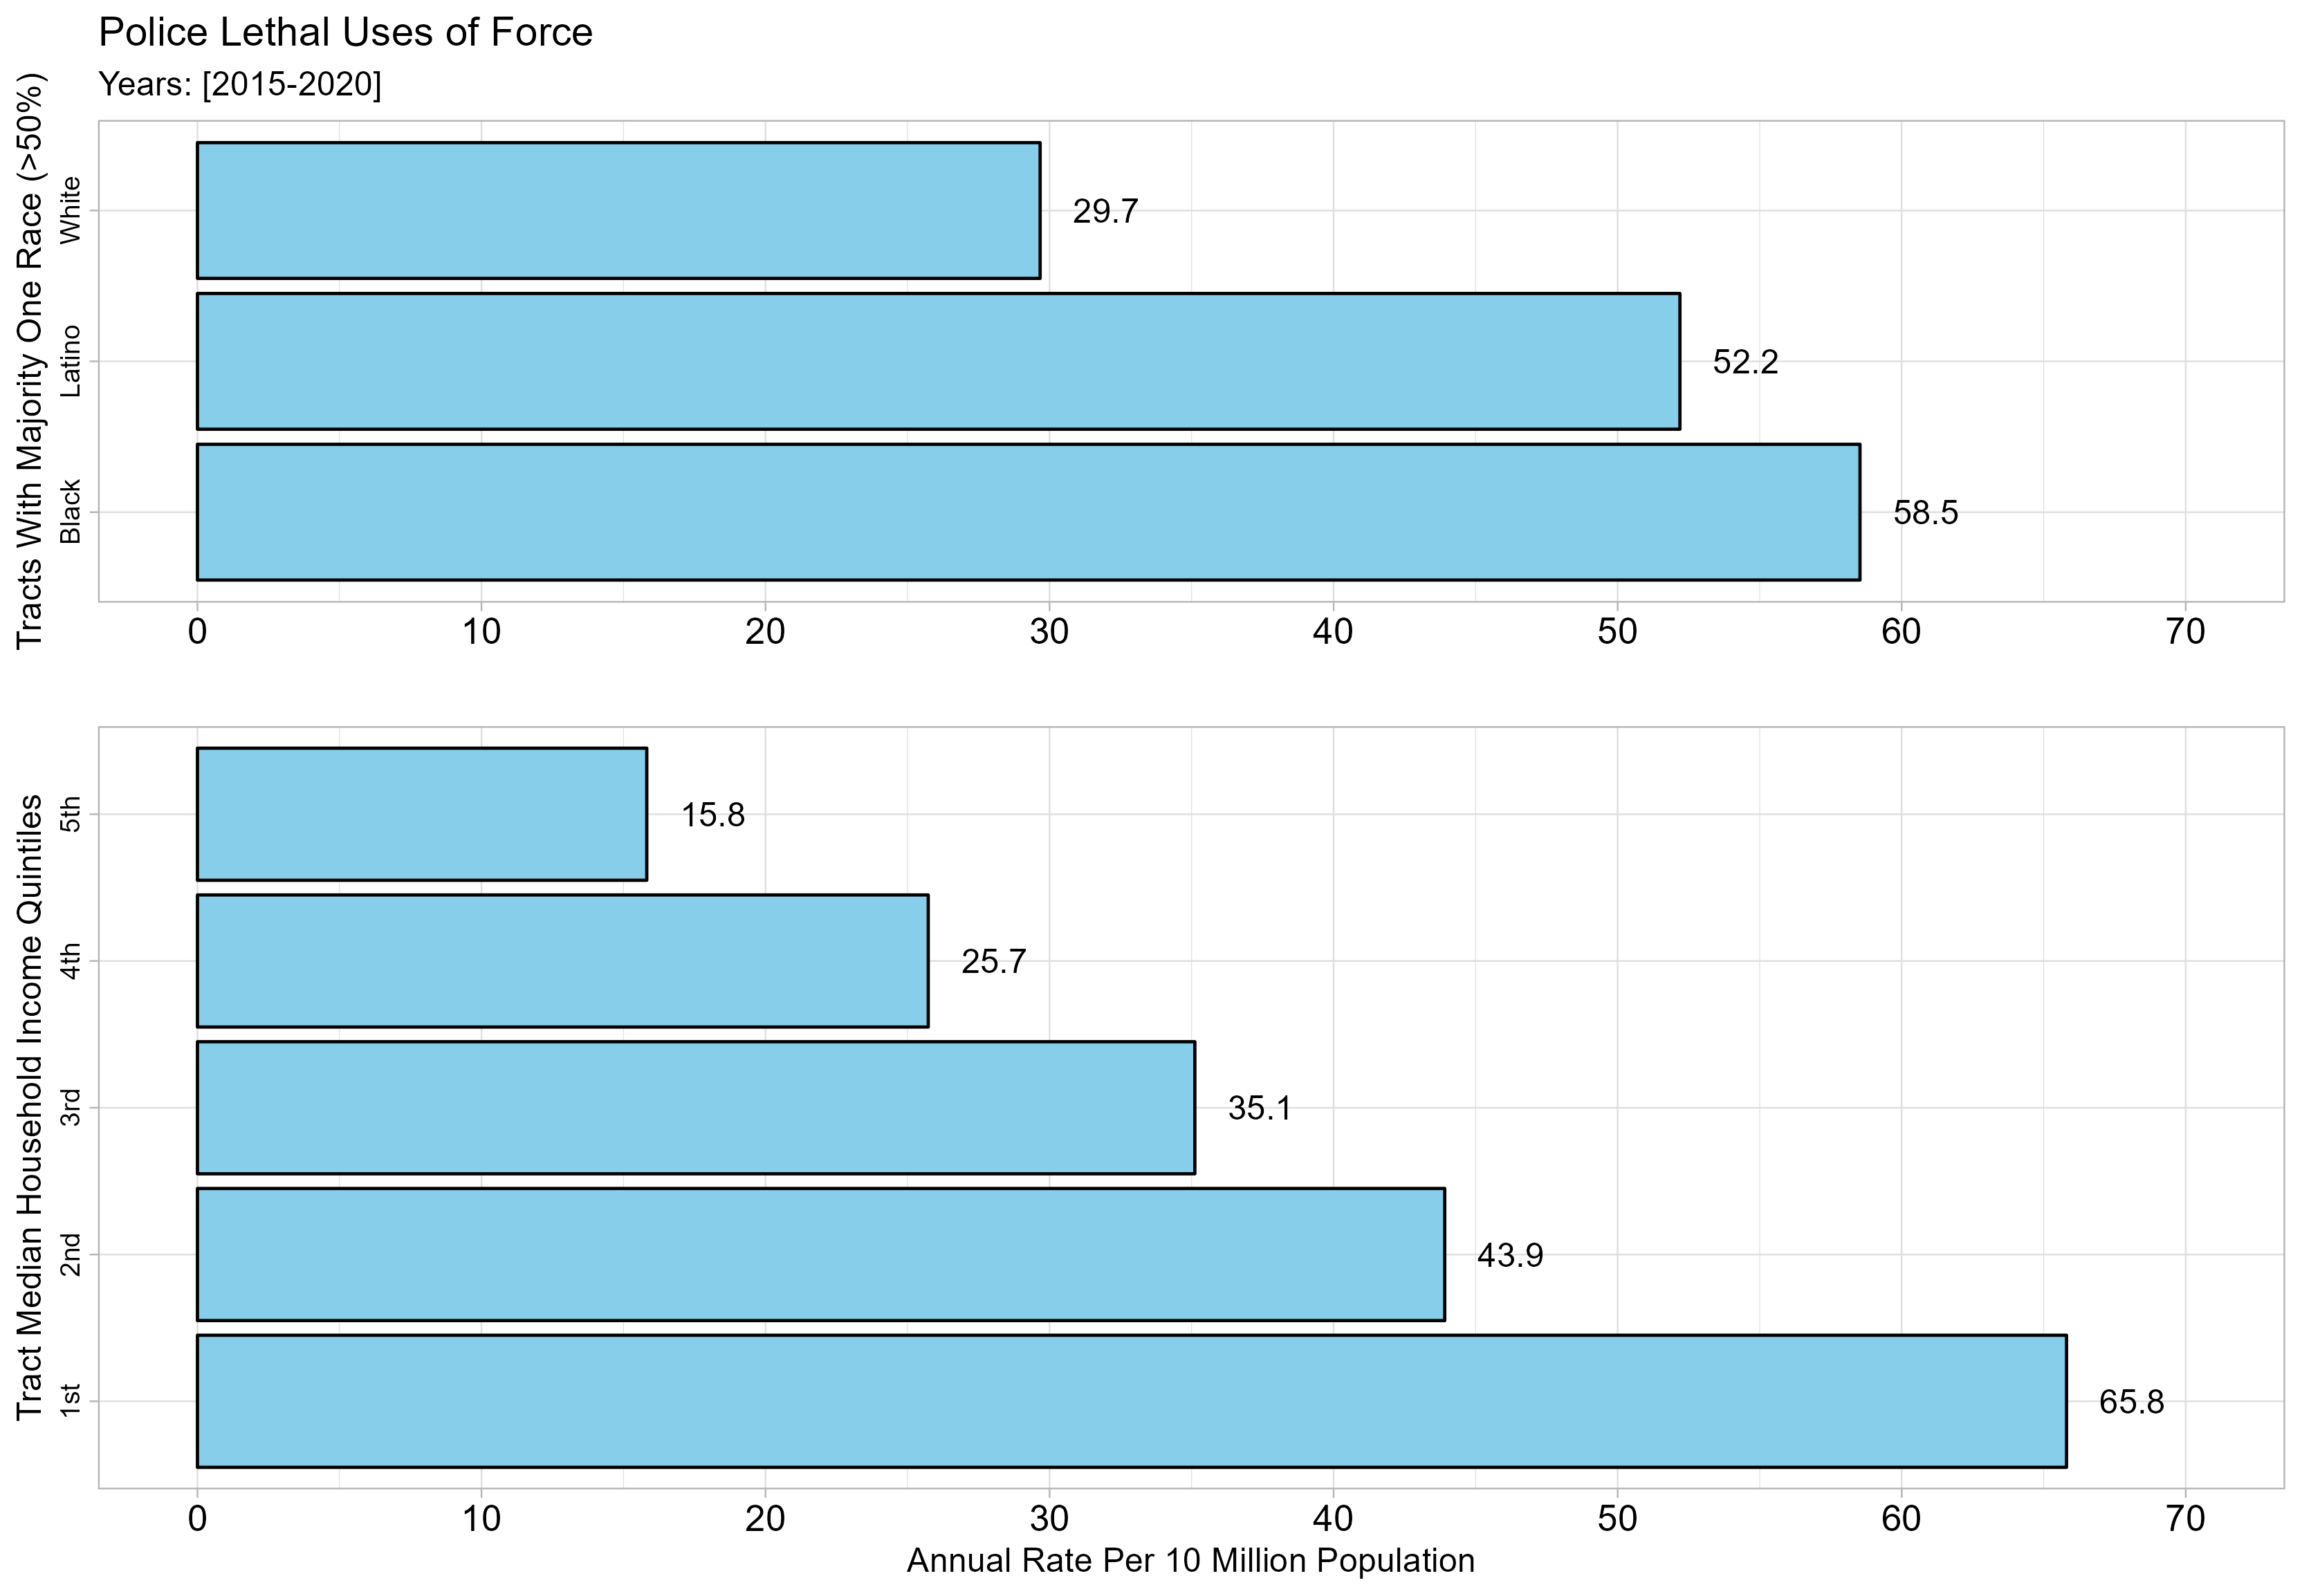
\includegraphics[height=0.8\textheight]{images/combined}	
	\end{center}
	\note[item]{Majority-black neighborhoods experience a rate nearly twice that of majority-white neighborhoods.}
	\note[item]{Majority-Hispanic/Latino neighborhoods experience a rate 1.75 times greater than majority-white neighborhoods.}
	\note[item]{US census tracts were binned into quintiles based on the distribution of median household income across all US census tracts.}
	\note[item]{Median household income has a strong relationship with the rate of police killings.}
	\note[item]{Police killings occur at the greatest frequency in the lowest-income tracts.}
	\note[item]{The lowest household income quintile tracts experience a rate over four times that of the highest household income tracts.}
%	\vspace*{24pt}
\end{frame}

%\begin{frame}{Findings: Median Household Income}
%	\begin{center}
%	\includegraphics[width=0.5\linewidth]{images/income_quintiles_only}
%	\end{center}
%	\vspace*{24pt}
%\end{frame}

\begin{frame}{Findings: Median Household Income}
	\begin{center}
		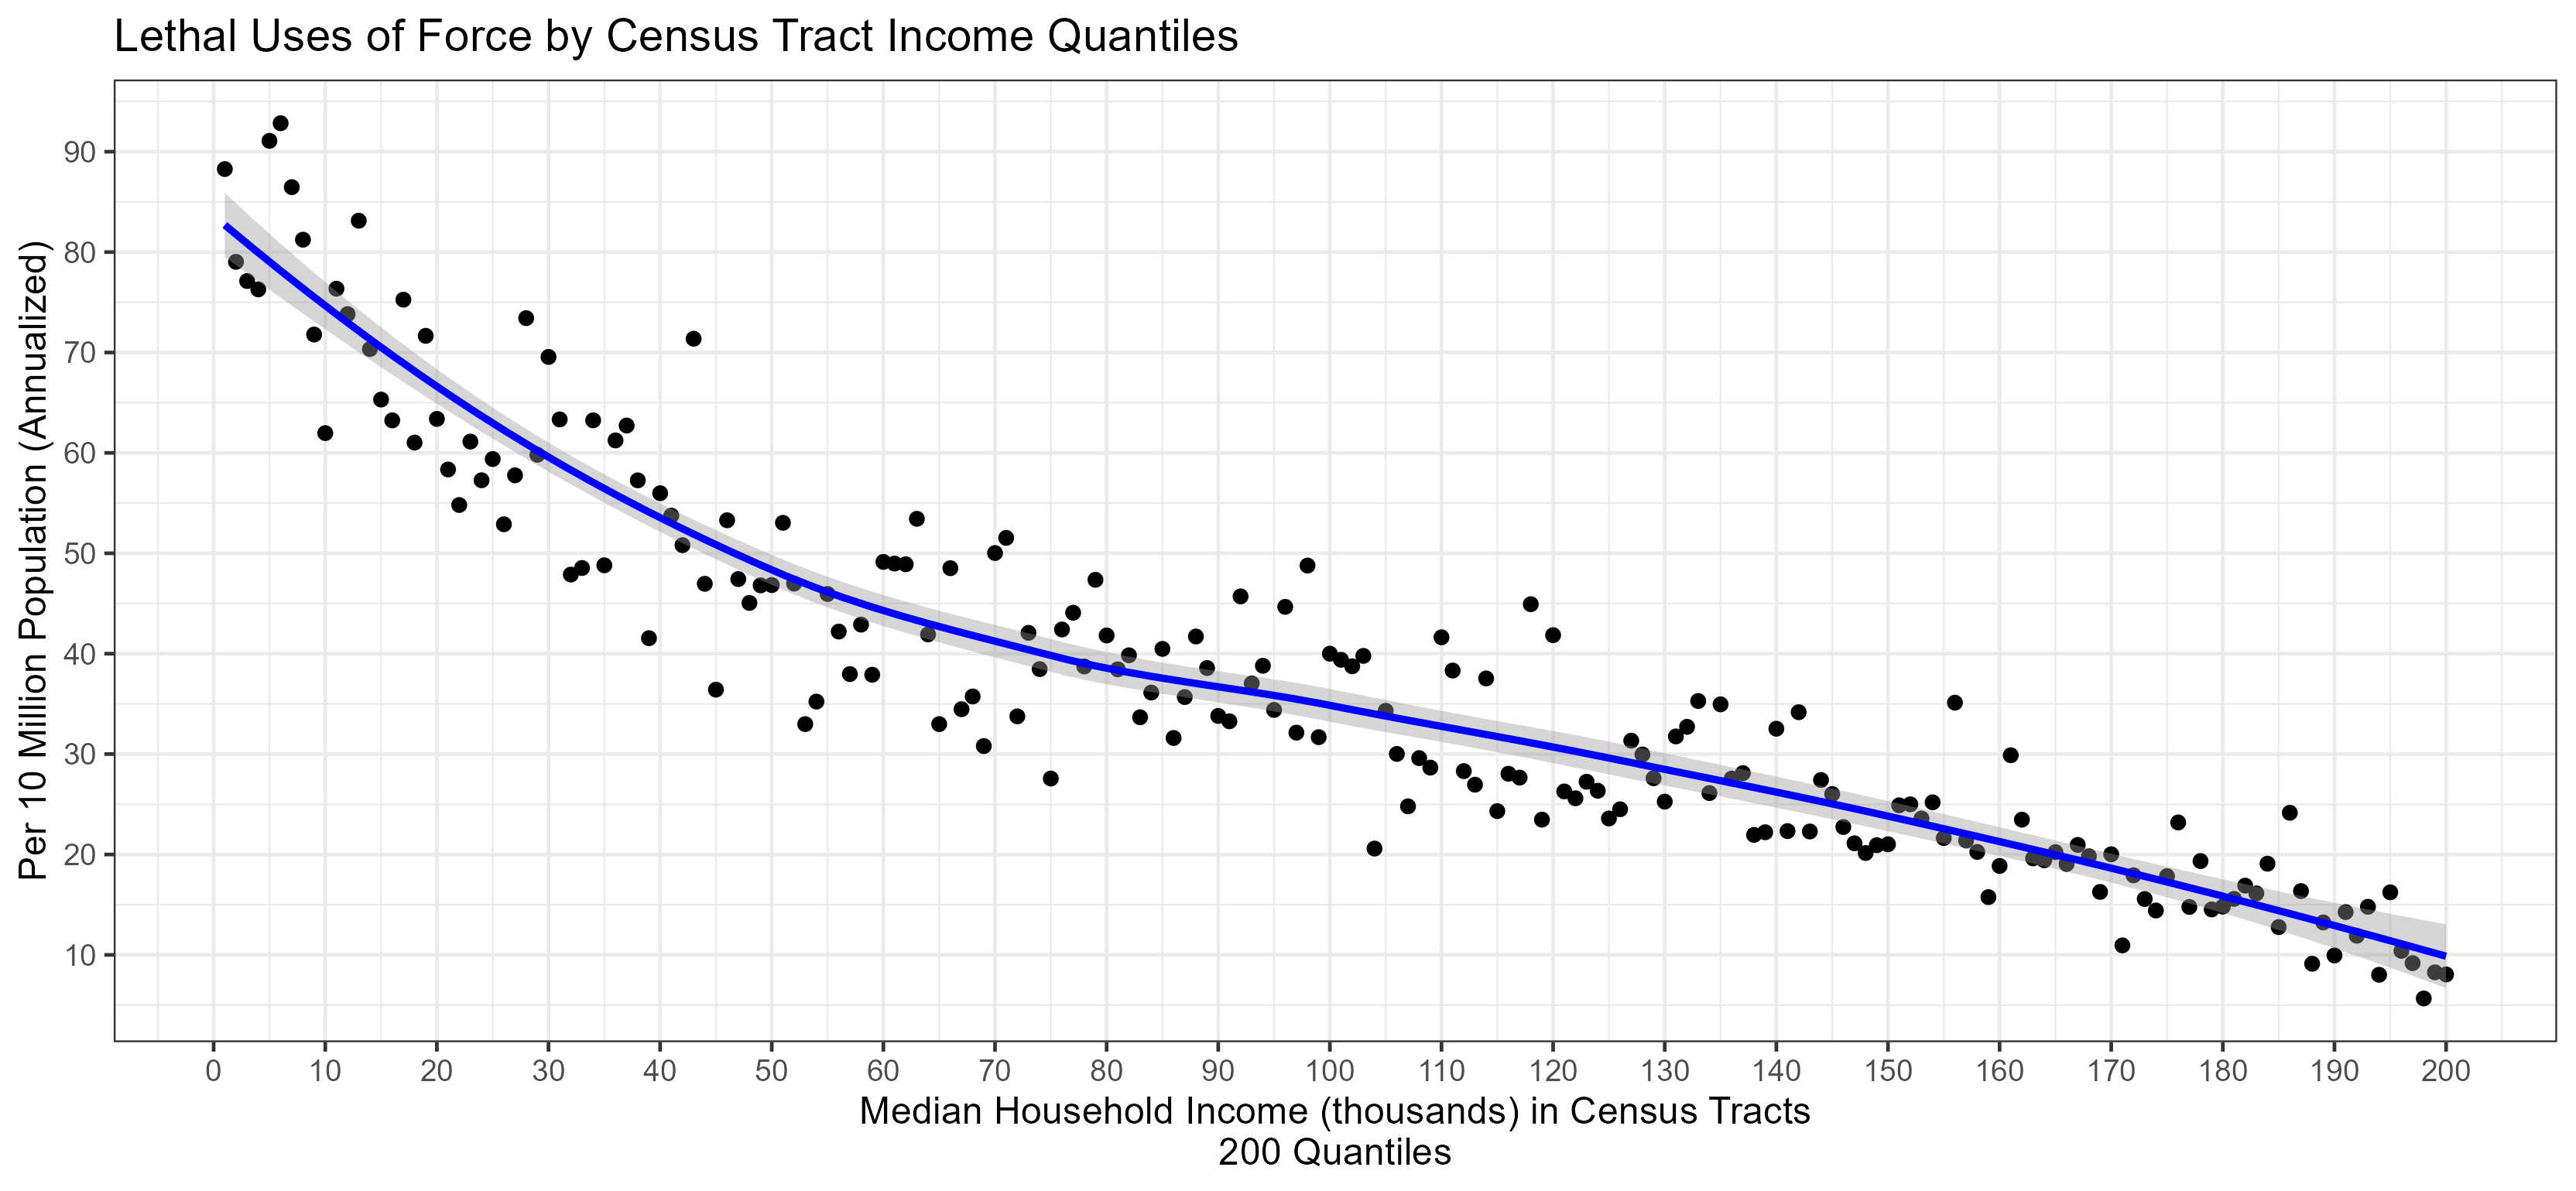
\includegraphics[width=\linewidth]{images/all_200}
	\end{center}
\end{frame}

\begin{frame}{Findings: Majority Race and Income}
	\begin{center}
		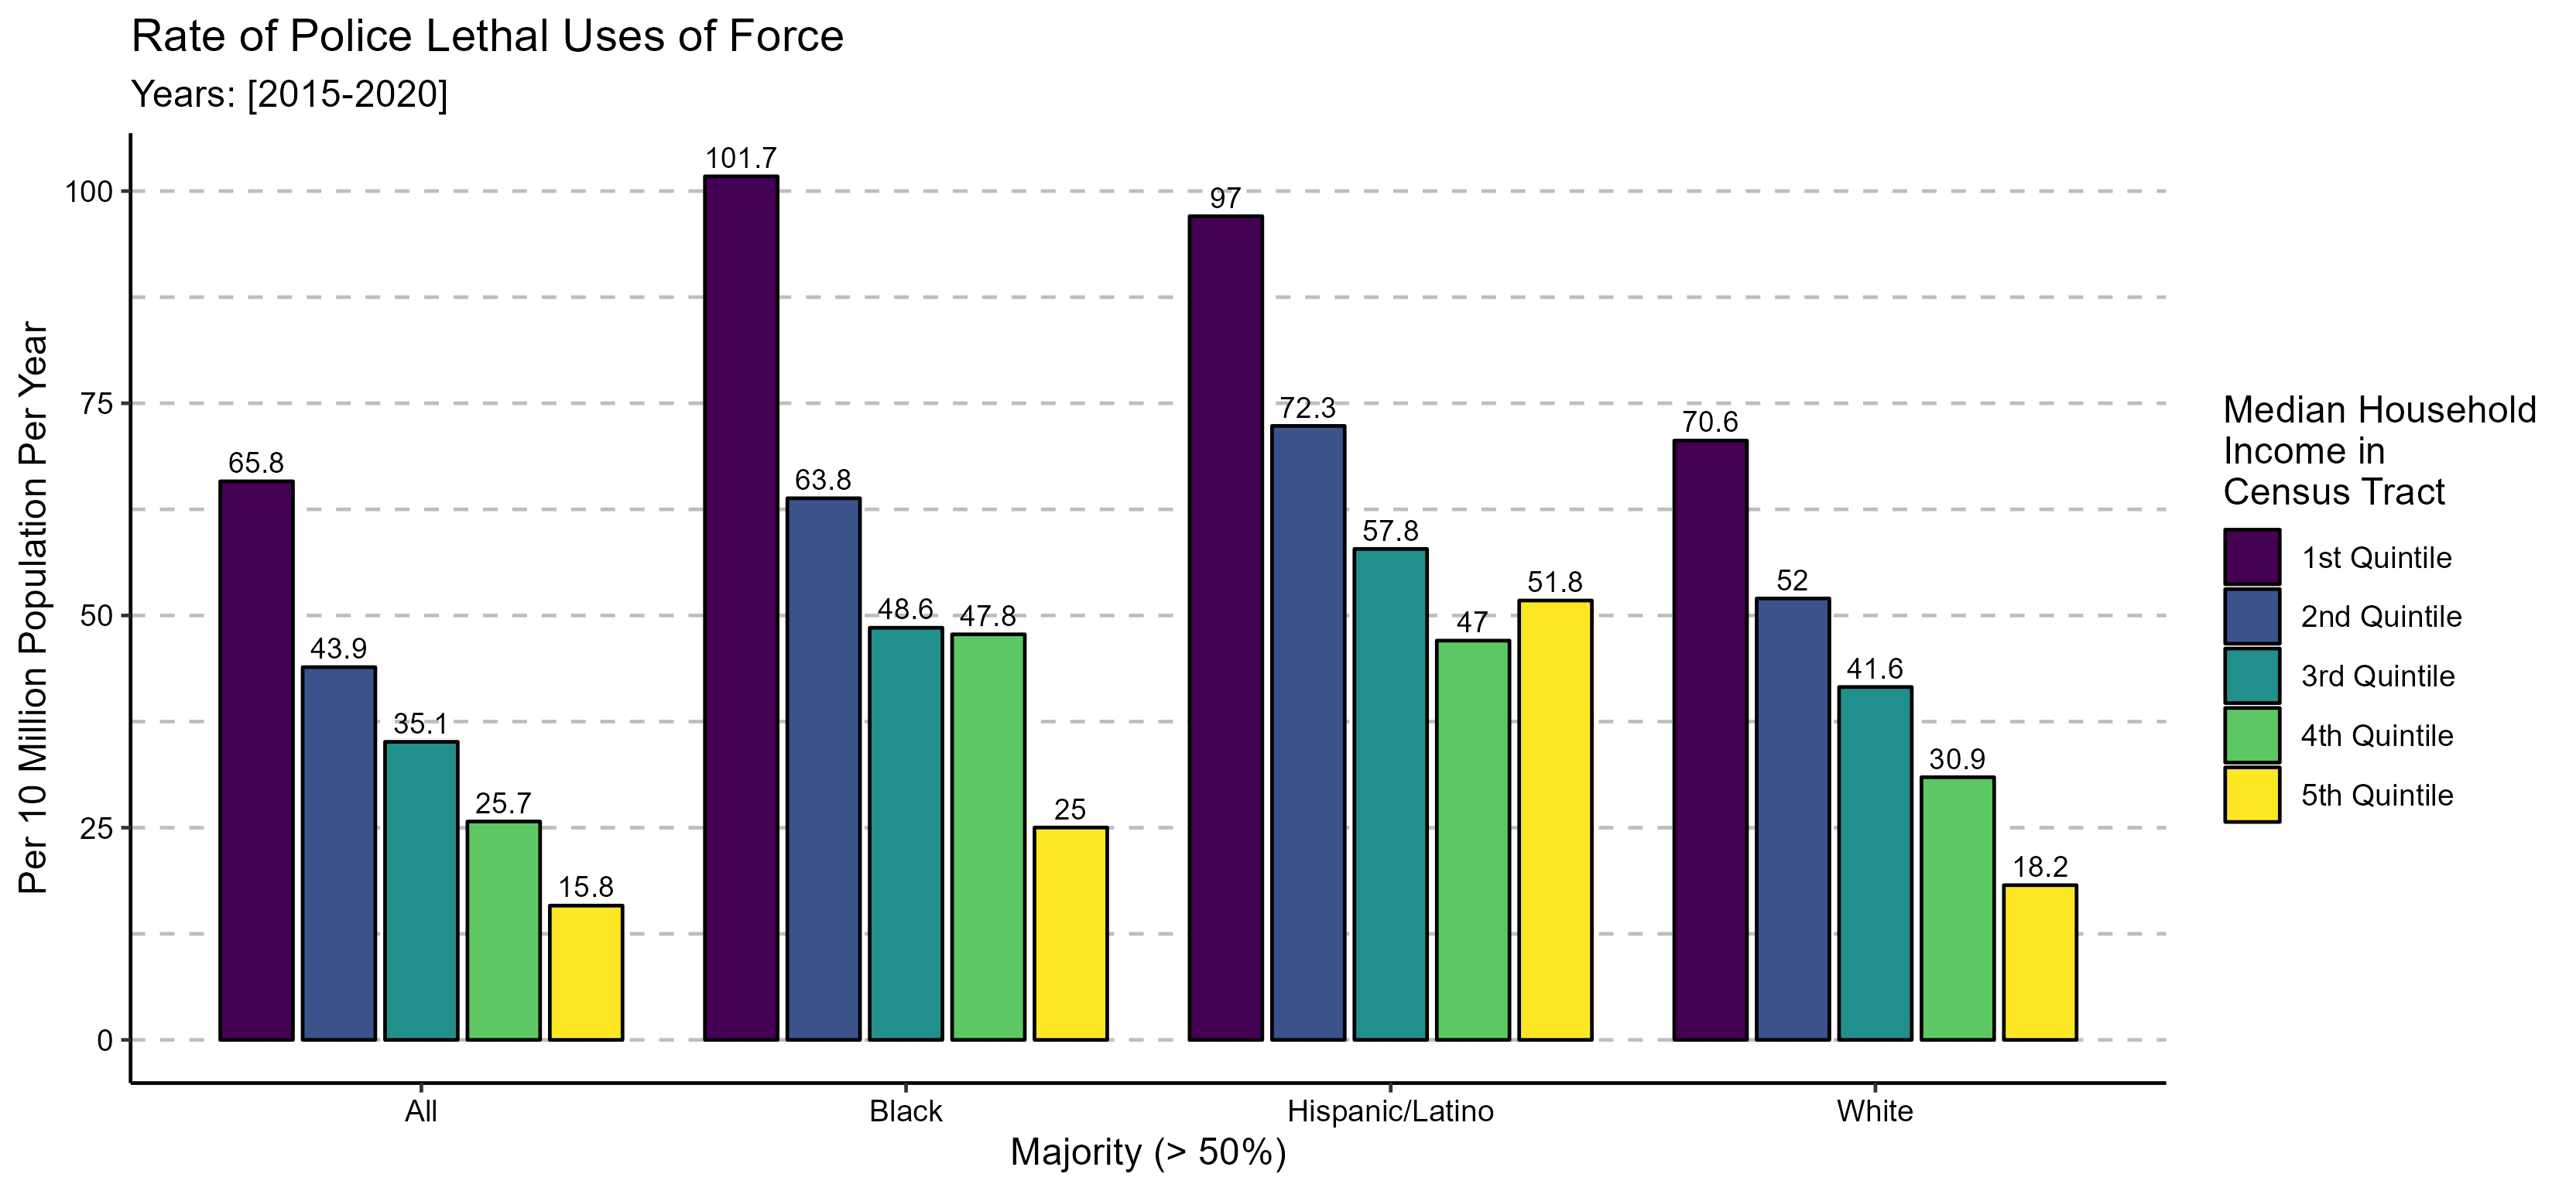
\includegraphics[width=\linewidth]{images/race_only_denom_race}
	\end{center}
\end{frame}

\begin{frame}{Logistic Regression: Income Only}
    \begin{columns}
        % First column for the table
        \begin{column}{0.5\textwidth}
        	\resizebox{\linewidth}{!}{%
                \begin{tabular}{lcccccc}
                    \toprule
                    Log likelihood: & -21947.515 & & & & & \\
                    \midrule
                    \multicolumn{3}{l}{Number of obs: 82,907} & \multicolumn{4}{l}{LR chi2(1): 875.58} \\
                    \multicolumn{3}{l}{Prob $>$ chi2: 0.0000} & \multicolumn{4}{l}{Pseudo R2: 0.0196} \\
                    \midrule
                    \midrule
                    \texttt{fatal\_enc\_binary} & Coefficient & Std. err. & z & P$>|$z$|$ & \multicolumn{2}{c}{[95\% conf. interval]} \\
                    \midrule
                    \texttt{IncomeE\_1k} & -0.013265 & 0.0004899 & -27.08 & 0.000 & -0.0142252 & -0.0123049 \\
                    \texttt{\_cons} & -1.636736 & 0.0319747 & -51.19 & 0.000 & -1.699406 & -1.574067 \\
                    \bottomrule
                \end{tabular}
			}
        \end{column}

        % Second column for the image
        \begin{column}{0.5\textwidth}
            \centering
            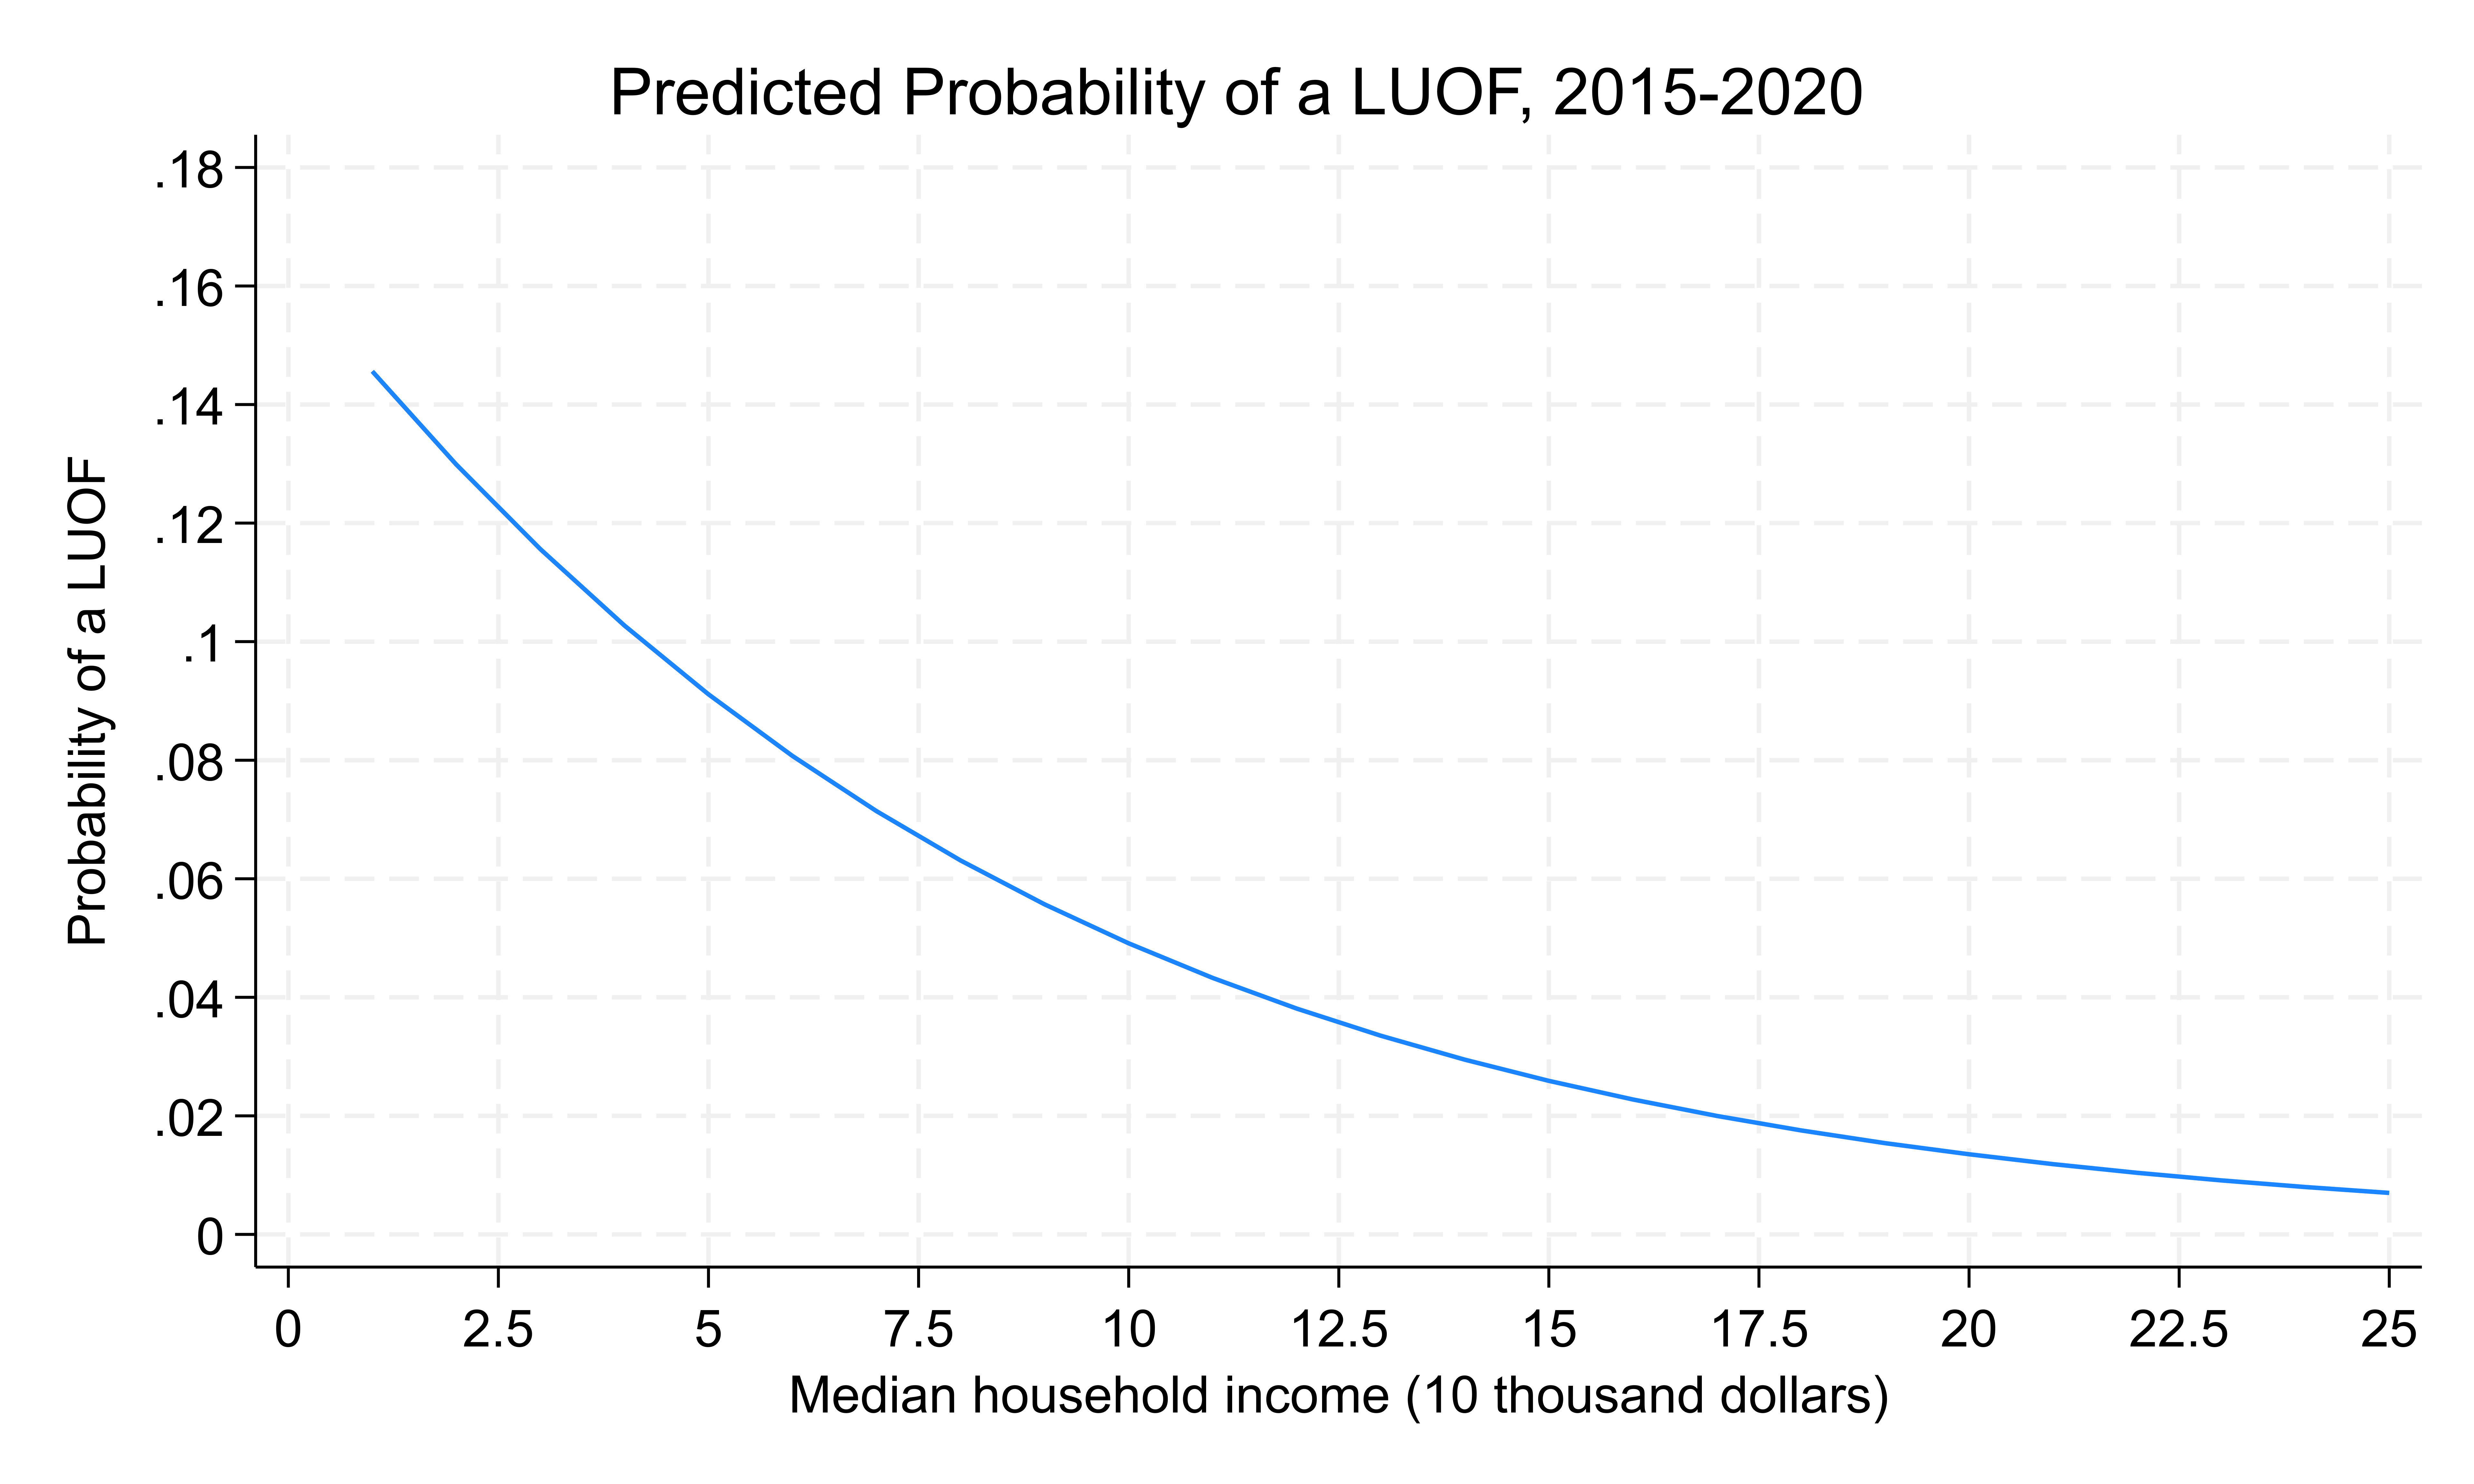
\includegraphics[width=\linewidth]{images/LUOF_logit_income_only}
        \end{column}
    \end{columns}
\end{frame}

\begin{frame}{Logistic Regressions: Race/Ethnicity}
	\begin{center}
	\includegraphics[height=0.9\textheight]{images/LUOF_logit_race}
	\end{center}
\end{frame}

\begin{frame}{Logistic Regressions: Marginal Effects}
	\begin{center}
		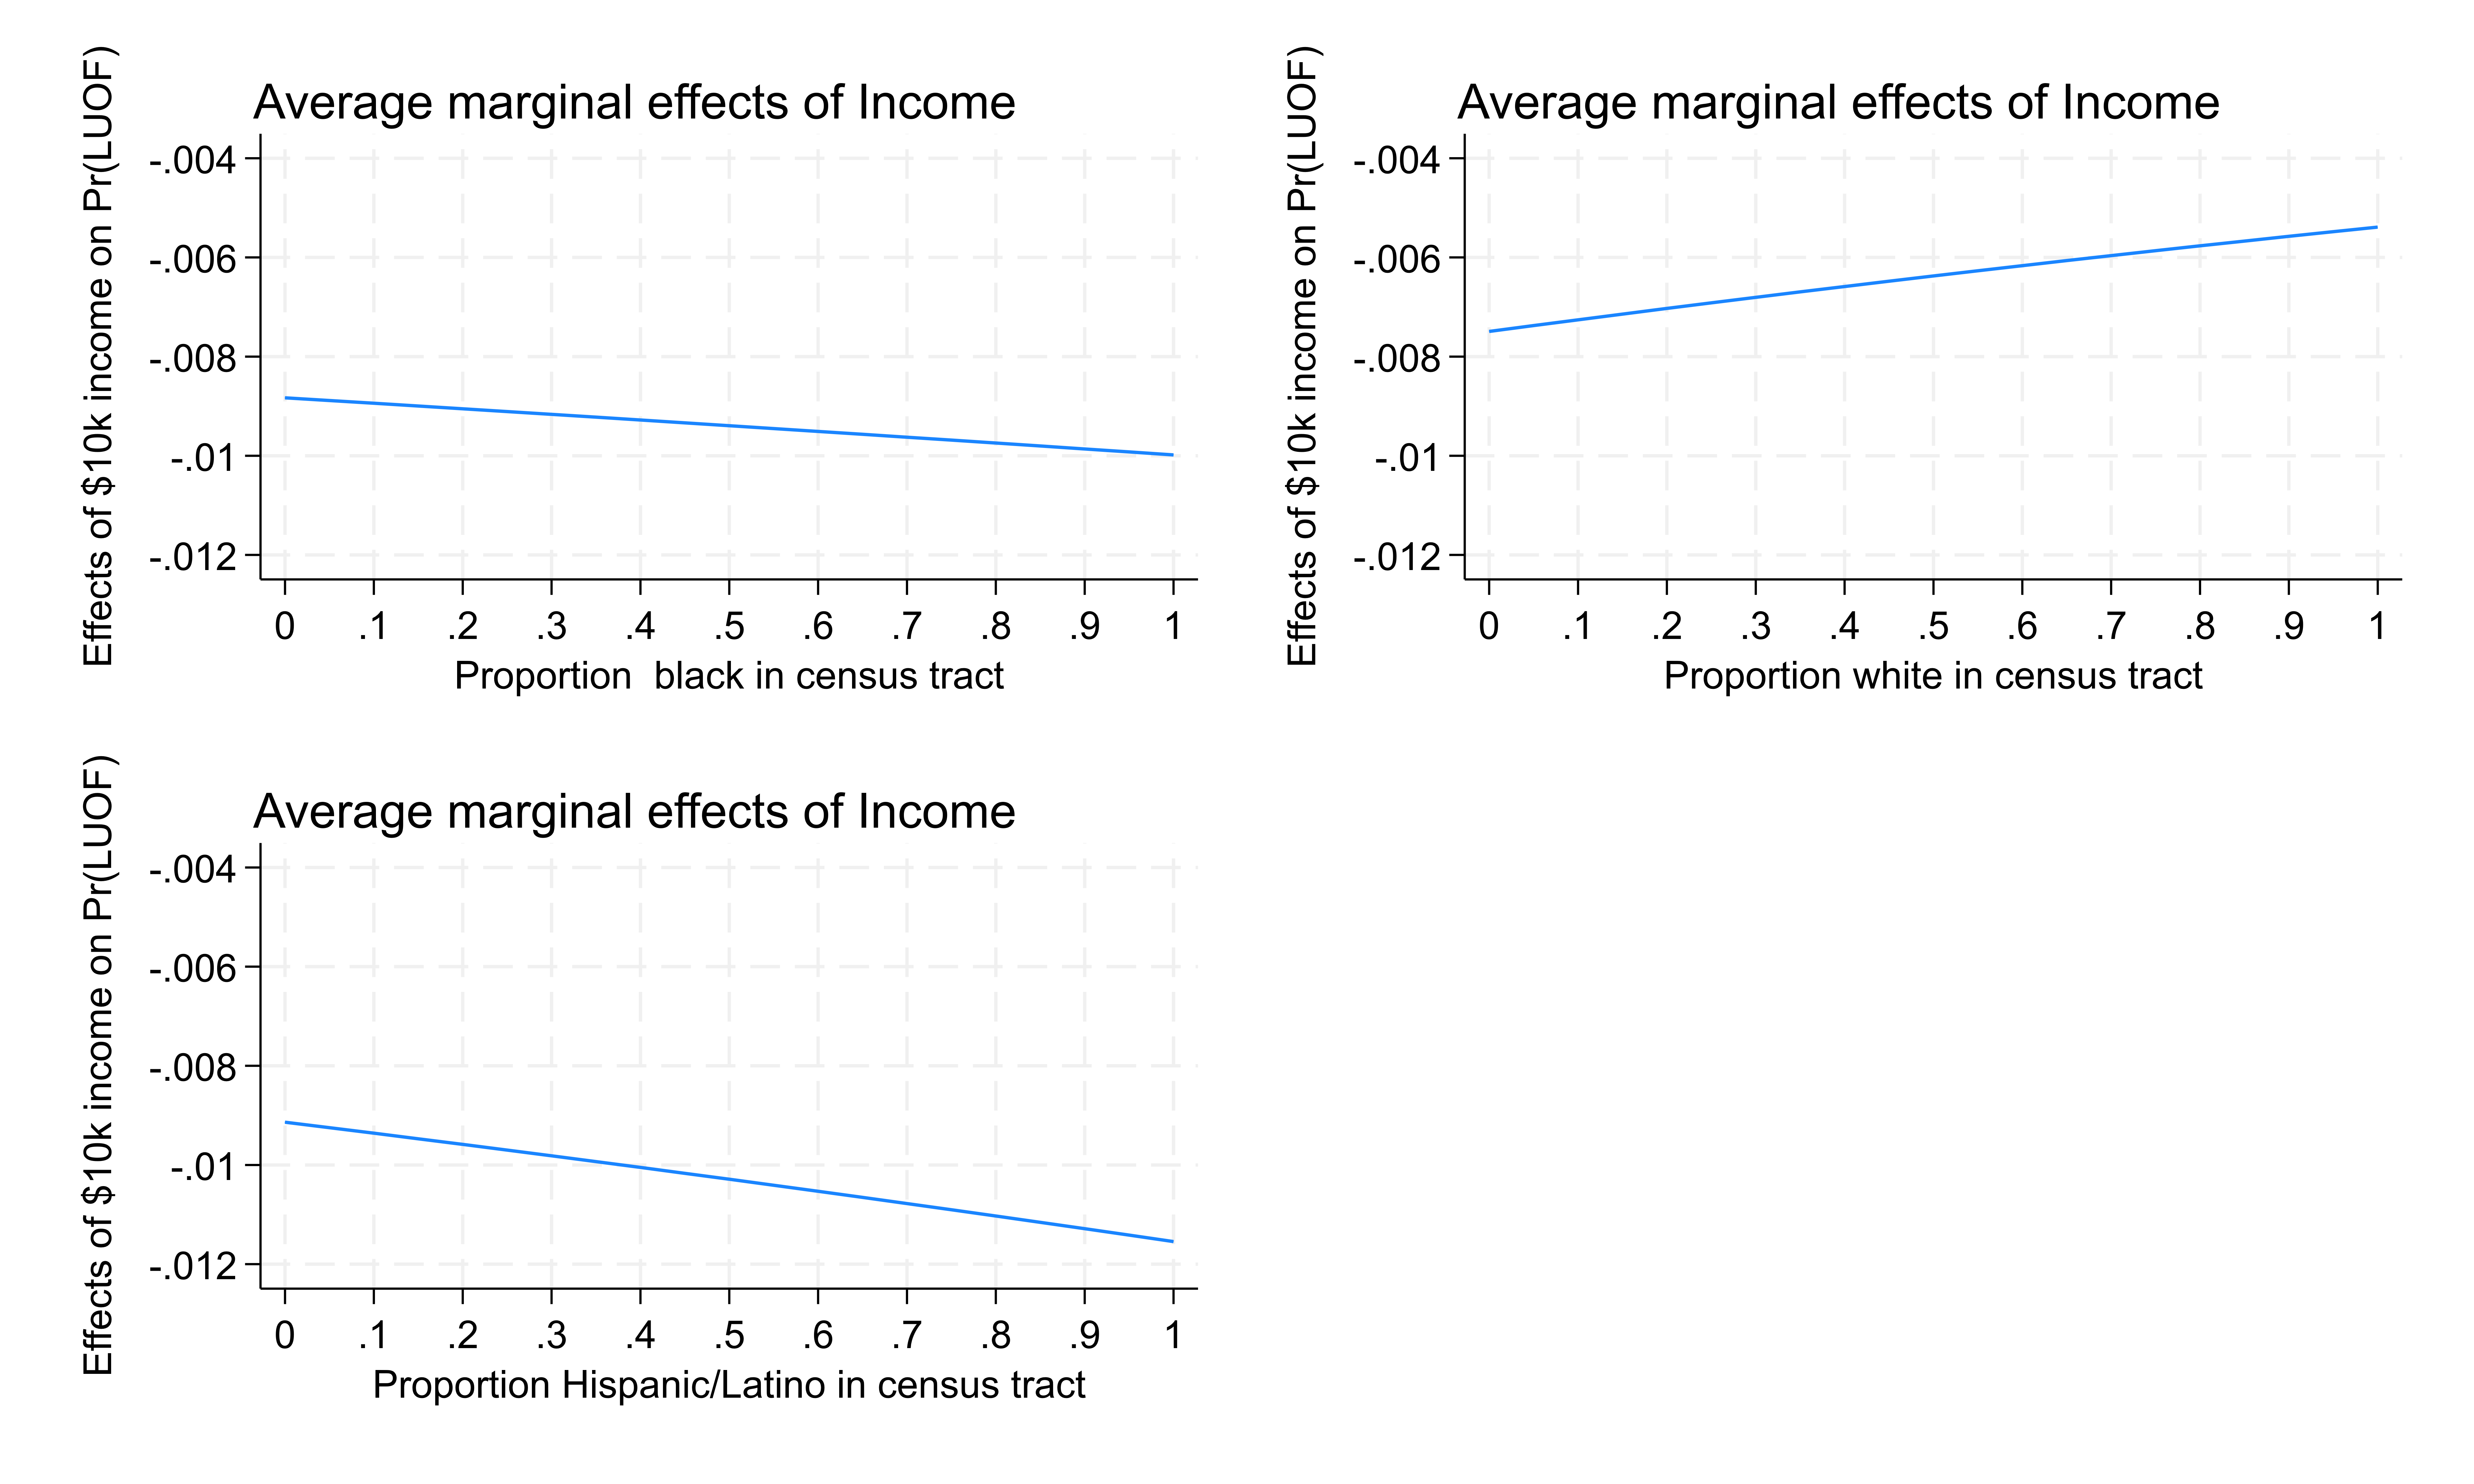
\includegraphics[height=0.9\textheight]{images/LUOF_logit_combined_effects}
	\end{center}
\end{frame}

%----- Gentrification -----%
\section{Findings: Gentrification}
\begin{frame}{Gentrification and Victims’ Race}
	Text goes here\ldots
\end{frame}

\begin{frame}{Gentrification and Majority Race}
	Text goes here\ldots
\end{frame}

\begin{frame}{Gentrification, Majority Race and Victim’s Race}
	Text goes here\ldots
\end{frame}

%----- Discussion -----%
\section{Discussion}
\begin{frame}{Findings: Discussion}
	Text goes here\ldots
\end{frame}

%----- Limitations and Future Research -----%
\begin{frame}{Limitations and Future Research}
	Text goes here\ldots
\end{frame}


\sloppy
\begin{frame}{Bibliography}
%	\fontsize{4}{7.2}\selectfont
	\printbibliography
\end{frame}

%\begin{frame}{Racial Disparities}
%\begin{itemize}
%\begin{tabular}{|c|c|c|}
%  \hline
%  Header 1 & Header 2 & Header 3 \\
%  \hline
%  Row 1, Cell 1 & Row 1, Cell 2 & Row 1, Cell 3 \\
%  \hline
%  Row 2, Cell 1 & Row 2, Cell 2 & Row 2, Cell 3 \\
%  \hline
%\end{tabular}
%\end{itemize}
%\end{frame}

\end{document}